\section{Part\-Two\-Opt\-Init Class Reference}
\label{class_part_two_opt_init}\index{PartTwoOptInit@{PartTwoOptInit}}
It sets the first couple of edges.  


{\tt \#include $<$part\_\-two\_\-opt\_\-init.h$>$}

Inheritance diagram for Part\-Two\-Opt\-Init::\begin{figure}[H]
\begin{center}
\leavevmode
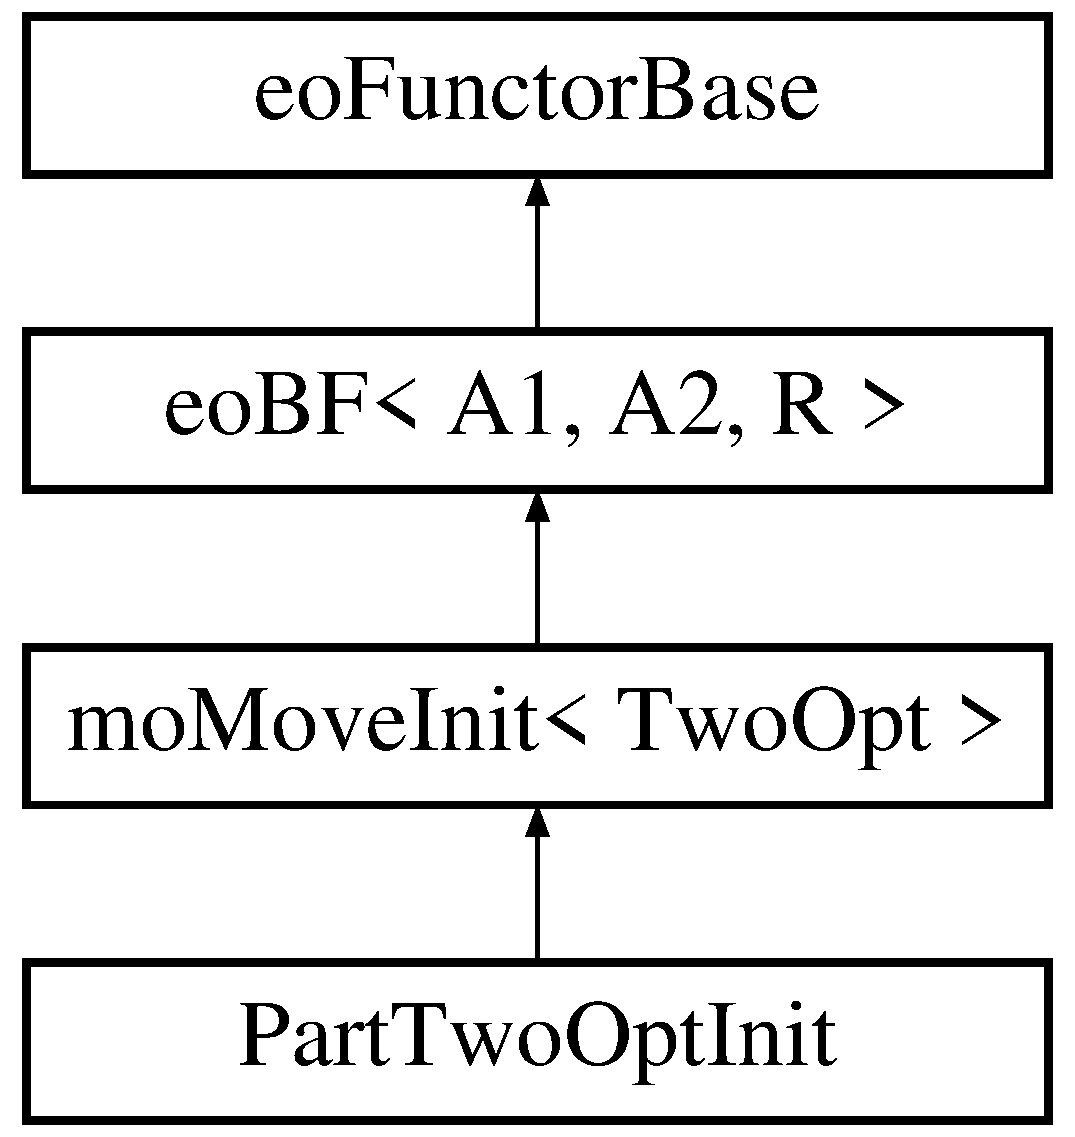
\includegraphics[height=4cm]{class_part_two_opt_init}
\end{center}
\end{figure}
\subsection*{Public Member Functions}
\begin{CompactItemize}
\item 
void \bf{operator()} (\bf{Two\-Opt} \&\_\-\_\-move, const \bf{Route} \&\_\-\_\-route)\label{class_part_two_opt_init_2f6190b1700ca1a12d0baaceaf75383c}

\end{CompactItemize}


\subsection{Detailed Description}
It sets the first couple of edges. 



Definition at line 45 of file part\_\-two\_\-opt\_\-init.h.

The documentation for this class was generated from the following files:\begin{CompactItemize}
\item 
part\_\-two\_\-opt\_\-init.h\item 
part\_\-two\_\-opt\_\-init.cpp\end{CompactItemize}
